\documentclass[a4paper, 11pt]{article}
\usepackage[french]{babel}
\usepackage[utf8]{inputenc}
\usepackage[T1]{fontenc}
\usepackage{datetime}
\usepackage{float}
\usepackage{eurosym}
\usepackage{comment} % enables the use of multi-line comments (\ifx \fi)
\usepackage{graphicx}
\usepackage{eurosym}
\usepackage{rotating}
\usepackage{enumitem}
\usepackage[style=long,nonumberlist,toc,xindy,acronym,nomain]{glossaries} % glossary with acronyms

\usepackage{mdframed}
\mdfdefinestyle{HighlightQuestion}{
  linecolor=red,
  linewidth=2pt,
  roundcorner=5
}

\usepackage{framed, color} % shade-box around the text to highlight
\definecolor{shadecolor}{RGB}{211,211,211}

\usepackage{fullpage} % changes the margin

\setlist[itemize,1]{label={$\bullet$}}
\makenoidxglossaries
\setlength{\glsdescwidth}{0.8\linewidth} % Wider glossary section
\renewcommand{\glsnamefont}[1]{\textbf{#1}}
\renewcommand{\glossarysection}[2][]{} % Do not print glossary title
\input{glossary.gloss}
\begin{document}



\begin{titlepage}

\newcommand{\HRule}{\rule{\linewidth}{0.5mm}} % Defines a new command for the horizontal lines, change thickness here

\center % Center everything on the page
%----------------------------------------------------------------------------------------
%	HEADING SECTIONS
%----------------------------------------------------------------------------------------

\textsc{\LARGE Université catholique de Louvain \\ École Polytechnique de Louvain}

\vfill


\includegraphics[scale=0.45]{Cahier_des_Charges/epl.jpg}

\vfill

% \textsc{\Large Mémoire 2018-2019}\\[0.5cm] % Major heading such as course name
\textsc{\large Gestion de la distribution d'eau en Haïti}\\[0.5cm] % Minor heading such as course title

%----------------------------------------------------------------------------------------
%	TITLE SECTION
%----------------------------------------------------------------------------------------

\HRule \\[0.5cm]
{ \huge \bfseries Cahier des Charges}\\[0.3cm] % Title of your document
\HRule

\vfill

%----------------------------------------------------------------------------------------
%	AUTHOR SECTION
%----------------------------------------------------------------------------------------

\begin{minipage}[t]{0.4\textwidth}
\begin{flushleft} \large
\emph{Auteurs:}\\
\textsc{Deknop} Céline \\
\textsc{Hallet} Adrien \\
\textsc{Strebelle} Sébastien \\
\end{flushleft}
\end{minipage}
~
\begin{minipage}[t]{0.4\textwidth}
\begin{flushright} \large
\emph{Promoteurs:} \\
\textsc{Pr. Mens} Kim \\
\textsc{Pr. Soares-Frazão} Sandra \\% Supervisor's Name
\end{flushright}
\end{minipage}

% If you don't want a supervisor, uncomment the two lines below and remove the section above
%\Large \emph{Author:}\\
%John \textsc{Smith}\\[3cm] % Your name
\vfill
%----------------------------------------------------------------------------------------
%	DATE SECTION
%----------------------------------------------------------------------------------------

{\large \today} % Date, change the \today to a set date if you want to be precise

%----------------------------------------------------------------------------------------
%	LOGO SECTION
%----------------------------------------------------------------------------------------

% Include a department/university logo - this will require the graphicx package

%----------------------------------------------------------------------------------------
\end{titlepage}
\title{Assignment 1 - Modeling phase}
\newpage

\section{Glossaire}
  \printnoidxglossary
\section{Introduction}

L'ONG Protos\footnote{https://www.protos.ngo} nous a contactés afin que nous produisions une \gls{application} en ligne permettant de gérer le \gls{reseau} de distribution d'eau haïtien. Ce document expose les propositions pour la gestion des installations, \glspl{consommateur} et finances du \gls{reseau}.

Nous débutons par une exposition des propositions d'\glspl{utilisateur} et fonctionnalités qui expliquent le principe de fonctionnement de l'\gls{application}. Ensuite, quelques ébauches (non-exhaustives) de l'\gls{interface} graphique permettent de comprendre les propositions en pratique. Enfin, quelques informations pratiques vous informent de notre démarche dans ce projet.

Vous êtes invités à réagir à ce cahier des charges pour l'ajout et la modification de toute fonctionnalité qui vous semblerait manquante ou incohérente. Des sections \emph{Questions et Remarques} sont d'ailleurs présentes pour attirer votre attention sur certains points pour lesquels nous nécessitons des précisions. Ce sont des points importants mais la totalité du document est soumise à votre approbation.

\section{Types d'\glspl{utilisateur}}
\label{users}
Cette section du document contient une description détaillée de tous les types d'\glspl{utilisateur} qui, à terme, interagiront avec l'\gls{application}. Nous détaillons aussi ce que ceux-ci pourront faire avec l'\gls{application}, pour vous donner un contexte.

  \begin{description}
    \item[Gestionnaire de \glspl{fontaine}] est un type d'\gls{utilisateur} auquel on assigne un ou plusieurs éléments du \gls{reseau} de distribution de type "sortie" (\gls{fontaine}, \gls{kiosque}, \gls{reservoir}, branchement individuel) dont il est responsable.
    Il gère également la gestion des \glspl{consommateur} d'eau dans sa \gls{zone} et les ajoute/supprime/modifie dans le \gls{systeme} lorsque c'est nécessaire (naissance, décès, déménagement).
    Il utilise l'\gls{application} pour signaler des problèmes et ainsi pouvoir en avertir le technicien/plombier et sa hiérarchie. Chaque mois, le gestionnaire de \glspl{fontaine} utilise l'\gls{application} pour déposer un rapport. Ce rapport contient, pour chaque \gls{element_reseau} sous sa responsabilité, les quantités d'eau distribuées (si un compteur est présent), les recettes (\gls{htg}), l'état (en service, hors service). Une section générale (une seule fois par rapport) déclare également les heures et jours de service du gestionnaire de \glspl{fontaine}.

    \emph{Exemple : une personne chargée de gérer un \gls{point_eau} pourrait être un gestionnaire de \glspl{fontaine}. Il peut ainsi utiliser l'\gls{application} pour envoyer mensuellement les \glspl{donnee}, ajouter les \glspl{utilisateur} lorsque nécessaire et déclarer les problèmes.}

    \item[Gestionnaire de \gls{zone}] est un type d'\gls{utilisateur} qui gère un groupe de gestionnaires de \glspl{fontaine}. Il dispose des mêmes \glspl{permission} que les gestionnaires de \glspl{fontaine} dans sa \gls{zone} et peut donc effectuer les mêmes actions avec l'\gls{application}. En plus, le gestionnaire de \gls{zone} peut créer et supprimer des \glspl{utilisateur} "gestionnaire de \glspl{fontaine}" et  "techniciens/plombiers" et leur assigner des \glspl{permission} sur les éléments du \gls{reseau}. Le gestionnaire de \gls{zone} peut également créer, supprimer et modifier des éléments du \gls{reseau}.

    \emph{Exemple 1 : Protos ou la \gls{dinepa} peuvent être assignées en tant que gestionnaires de \gls{zone} ayant les accès sur tous les \gls{systeme}s et agir en tant que gestionnaires généraux de tout le \gls{systeme}. Ils peuvent donc consulter toutes les informations rapportées par les autres \glspl{utilisateur}.}

    \emph{Exemple 2 : un \gls{caepa} pourrait être assigné en tant que gestionnaire de \gls{zone} et avoir accès aux infrastructures du \gls{reseau} de distribution dans sa \gls{zone} géographique et ainsi consulter les informations et les modifier pour venir en aide aux gestionnaires de \glspl{fontaine}.}

    \item[\gls{consommateur}] est un type d'\gls{utilisateur} du \gls{reseau} de distribution d'eau, mais dans un premier temps, il n'aura pas accès à l'\gls{application}. Dans le futur (\emph{projet \gls{citizen_science} qui démarrera probablement en 2019-2020}), une nouvelle fonctionnalité de l'\gls{application} lui permettra de signaler un problème sur le \gls{reseau}, de consulter sa consommation (si applicable) et l'état du réseau et éventuellement d'autres fonctionnalités, qui seront détaillées par la suite.

    \item[Technicien/Plombier] est un type d'\gls{utilisateur} auquel on assigne des éléments du \gls{reseau} de distribution (\gls{fontaine}, \gls{reservoir}, \gls{prise_individuelle}, etc). Chaque technicien/plombier utilise l'\gls{application} pour voir les problèmes déclarés par les autres \glspl{utilisateur} (gestionnaires de \gls{fontaine}, de \gls{zone} ou \glspl{consommateur} quand le volet \emph{\gls{citizen_science}} sera ajouté). Il peut utiliser l'\gls{application} pour répondre aux demandes d'intervention, pour demander plus d'informations ou proposer une solution si le déplacement n'est pas nécessaire. Il peut modifier l'état d'un problème, demander des précisions et le marquer en cours de résolution ou résolu une fois l'intervention terminée.

    \emph{Exemple : un technicien/plombier démarrant sa journée peut consulter l'\gls{application} et voir quels sont les problèmes qui requièrent son attention. Il peut dialoguer avec les gestionnaires et modifier l'état des problèmes afin qu'à terme le \gls{reseau} fonctionne sans problème.}

  \end{description}
  \begin{mdframed}[style=HighlightQuestion]
    \subsection{Questions et remarques}
    % Questions
    \begin{enumerate}
      \item Le contenu du \gls{rapport_mensuel} d'un gestionaire de \gls{fontaine} est pour le moment basé sur le \gls{rapport_mensuel} existant (voir section~\ref{sec:approach}). Si vous souhaitez que l'\gls{application} récolte plus d'information auprès des gestionnaires, veuillez nous indiquer lesquelles et sous quelle forme (cela peut être un texte libre, un choix dans une liste, ce que vous voulez).
      \item Un gestionnaire de \gls{zone} dont la \gls{zone} recouvre tous les \gls{systeme}s peut être vu comme un administrateur et aurait dès lors \gls{acces_lecture} et \gls{acces_ecriture} à toutes les \glspl{donnee} de l'\gls{application}. Par erreur ou malveillance, il pourrait en effacer ou modifier certaines, faussant l'ensemble. Une pratique courante en informatique pour gérer ce problème potentiel est d'archiver les \glspl{donnee} : elles ne sont ainsi jamais vraiment modifiées ou effacées et peuvent être restaurées à l'état précédent. Est-ce une fonctionnalité que vous souhaitez pour l'\gls{application}, ou n'est-ce pas nécéssaire de s'en occuper ? Si ce modèle d'archivage ne vous convient pas, souhaitez-vous autre chose ?
      \item L'\gls{utilisateur} "technicien/plombier" et les fonctionnalités qui lui seront associées sont une interprétation de notre part car il nous semblait pratique de pouvoir centraliser la gestion du \gls{reseau} de distribution entièrement au sein de l'\gls{application}. Cela vous semble-t-il utile d'avoir une \gls{interface} destinée au technicien ?
    \end{enumerate}
  \end{mdframed}

  \section{Principe hiérarchique}
    L'\gls{application} fonctionne grâce à la hiérarchie de ses \glspl{utilisateur}. Cette hiérarchie se base sur la hiérarchie actuelle sur place tout en se voulant plus flexible pour accomoder d'éventuels cas particuliers et changements futurs.

    Ce principe est simple. Un gestionnaire de \glspl{fontaine} gère une ou plusieurs installations. Un gestionnaire de \gls{zone} gère un ou plusieurs gestionnaires de \gls{zone} et/ou de \glspl{fontaine}. En tant que gestionnaire de \gls{zone}, j'ai accès aux \glspl{donnee} des \glspl{utilisateur} que je gère. Si j'ajoute un \gls{element_reseau} ou un \gls{consommateur}, tous les \glspl{utilisateur} parents (\emph{i.e. : qui ont un lien hiérarchique vers le haut}) y ont accès également. Ce principe est illustré sur la figure \ref{fig:hierarchie}.

    \begin{figure}[H]
      \centering
      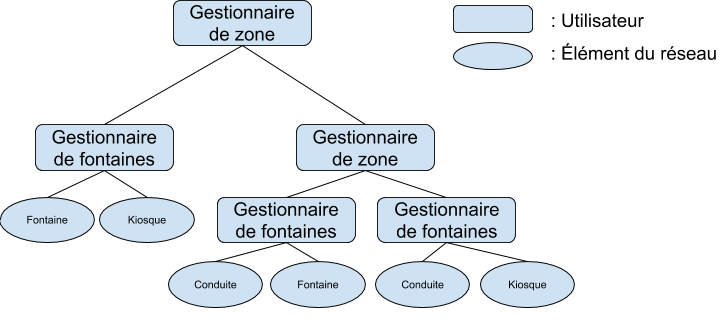
\includegraphics[width=.8\textwidth]{Cahier_des_Charges/principe_hierarchique}
      \caption{Exemple de hiérarchie}
      \label{fig:hierarchie}
    \end{figure}

    Les \glspl{consommateur} étant reliés aux \glspl{point_eau}, un \gls{utilisateur} n'a accès qu'aux \glspl{consommateur} et éléments du \gls{reseau} qui lui sont liés. Pour reprendre cet exemple, Protos pourrait être un gestionnaire de \gls{zone} en tête de liste et avoir accès à toutes les \glspl{donnee} collectées, tandis que le collectif gérant l'eau d'un village serait un gestionnaire de \glspl{fontaine} et ne pourrait consulter et modifier que les \glspl{donnee} dudit village. Ce \gls{systeme} permet une grande flexibilité dans la répartition des responsabilités.
\section{Fonctionnalités}
% Liste exhaustive des fonctionnalités de l'\gls{application}
% Séparer directement en fonction des différents \glspl{utilisateur} de l'\gls{application}

\subsection{Tout \gls{utilisateur} peut :}
\begin{itemize}
  \item Se connecter à l'\gls{application} via un identifiant et un mot de passe.
  \item Accéder aux pages de l'\gls{application} auxquelles il a accès en fonction de ses \glspl{permission} et de son type d'\gls{utilisateur} (gestionnaire de \gls{zone}, gestionnaire de \glspl{fontaine}, technicien/plombier).
  %\item Je peux effectuer mon travail hors ligne, pour l'envoyer plus tard quand j'aurai du \gls{reseau} % <- Impossible avec Django, on laisserait pas ça de côté pour le moment ? ça fait déjà beaucoup de travail et ils peuvent toujours noter sur leur pc et uploader quand ils ont une connexion
\end{itemize}

\subsection{Le gestionnaire de \gls{fontaine}(s) peut :}
\begin{itemize}
  \item Signaler un problème (matériel, qualité de l'eau, ...) à l'un des éléments du \gls{reseau} auquel il est assigné via \gls{ticket} pour que le technicien et ses supérieurs en soient informés. Le problème est modifiable (pour ajouter des détails par exemple) tant qu'il n'est pas cloturé.
  \item Clôturer un \gls{ticket} pour indiquer que le problème est résolu.
  \item Rentrer les \glspl{donnee} d'utilisation mensuelles correspondant aux \glspl{point_eau} auxquels il est assigné (\emph{cf section \ref{users} pour les détails du rapport}).
  \item Ajouter/supprimer/modifier un \gls{consommateur} (ou groupe de \glspl{consommateur} en indiquant le nombre de \glspl{consommateur} dans le foyer du chef de famille).
  \item Assigner un \gls{consommateur} ou groupe de \glspl{consommateur} à un \gls{point_eau}.
  \item Indiquer le montant payé par un \gls{consommateur} et pour quelle durée.
  \item Consulter l'état de recouvrement de son ou ses point(s) d'eau, obtenir les statistiques de recouvrement, lister les \glspl{consommateur} qui n'ont pas encore payé.
\end{itemize}

% Ils doivent également gérer les conflits, est-ce qu'on veut faire un pannel pour ça ou de la doc ou whatever ?

\subsection{Le gestionnaire de \gls{zone} peut :}
\begin{itemize}
  \item Visionner tous les éléments du \gls{reseau} la \gls{zone} et leurs informations (emplacement, \gls{utilisateur} responsable, état actuel, problèmes déclarés). Les informations pour un \gls{point_eau} sont plus nombreuses (statistiques sur le nombre d'\glspl{utilisateur}, débit mensuel, recettes mensuelles) que les informations d'un autre type d'élément (\emph{e.g. : une canalisation})
  \item Consulter toutes les \glspl{donnee} entrées par un gestionnaire de \gls{point_eau} (\glspl{rapport_mensuel}) dans la \gls{zone}.
  \item Consulter des graphiques générés automatiquement pour évaluer l'état du \gls{reseau}, des \glspl{utilisateur} et recouvrement dans la \gls{zone} assignée\footnote{Voir section Questions et remarques.}.
  \item Consulter les problèmes (\glspl{ticket}) déclarés dans la \gls{zone} assignée pour voir uniquement quels \glspl{point_eau} sont en difficulté.
  \item Assigner un technicien à un problème particulier pour le prioriser.
  \item Modifier l'état d'un \gls{ticket} pour en marquer la résolution ou la prise en charge.
  \item Agréger les \glspl{rapport_mensuel} pour obtenir des statistiques annuelles ou globales. %Pas trop spécifique à notre dernier document ? < hop, comme ça c'est réglé
  \item Créer ou supprimer des \glspl{utilisateur} (gestionaire de \glspl{fontaine}, gestionnaire de \gls{zone} ou technicien). %tricky les gestionnaires de \gls{zone} qui créent des gestionnaires de \gls{zone}
  \item Attribuer ou retirer un \gls{element_reseau}/\gls{zone} à un gestionaire de \glspl{fontaine}/\gls{zone}.
  \item Créer un \gls{element_reseau} dans sa \gls{zone}.
  \item Ajouter, modifier ou supprimer des dépenses et des revenus pour la \gls{zone}.
\end{itemize}

\subsection{Le technicien/plombier peut :}
\begin{itemize}
  \item Consulter les \glspl{ticket} du \gls{reseau} pour déterminer la nécessité d'intervenir ou non.
  \item Répondre aux \glspl{ticket} afin de demander des précisions ou donner des solutions (si le déplacement n'est pas nécessaire/possible).
  \item Modifier l'état d'un problème afin d'en indiquer la prise en charge ou résolution.
\end{itemize}

  \begin{mdframed}[style=HighlightQuestion]
    \subsection{Questions et remarques}
    \begin{enumerate}
      \item Pour les graphes et statistiques présentés aux gestionnaires de \glspl{fontaine} ou de \gls{zone}, nous en avons certains en tête, mais si quoi que ce soit vous semble peu utile ou qu'au contraire il manque quelque chose d'essentiel, il serait bon de le préciser :
      \begin{itemize}
        \item Nombre total de \glspl{fontaine} dans la \gls{zone}
        \item Nombre total d'\glspl{utilisateur} de ces \glspl{fontaine}
        \item Nombre de \glspl{consommateur} n'ayant pas encore payé sur cette période (période à déterminer)
        \item Répartition du type de \glspl{point_eau} (kiosques, \glspl{fontaine} ou \gls{prise_individuelle})
        \item Évolution du taux de recouvrement
      \end{itemize}
      \item La fonctionnalité des dépenses et revenus est pour le moment très flexible et permet d'ajouter des dépenses et entrées d'argent pour consulter le solde et l'évolution des dépenses au fil des mois/années. Nous avons peu d'informations sur le fonctionnement des budgets et les informations dont nous disposons actuellement ne nous permettent pas de créer un \gls{systeme} plus évolué.
      \item Lors du développement de l'\gls{application}, la priorité sera de créer le coeur de l'\gls{application} permettant de stocker et modifier les \glspl{donnee}. C'est sur cette base nécessaire que nous vous proposerons ensuite des outils plus avancés comme le \gls{systeme} d'information géographique qui permettra de visualiser le \gls{reseau} sur une carte interactive (type Google Maps).
      \item Vous constatez que le gestionnaire de \gls{zone} a un rôle important dans l'\gls{application} car il peut créer et modifier des éléments du \gls{reseau} ainsi que des \glspl{utilisateur} dans sa \gls{zone}. Dans l'\gls{application}, par défaut cela signifie que tout gestionnaire de \gls{zone} peut créer, supprimer et modifier les éléments du \gls{reseau} ou les \glspl{utilisateur}. Si vous trouvez que c'est une trop grosse responsabilité, on vous propose d'ajouter un paramètre spécial qui autorise ou refuse au gestionnaire de \gls{zone} la \textbf{création et suppression} des éléments du \gls{reseau} ou \glspl{utilisateur}. Grâce à ce paramètre, vous pourriez avoir des gestionnaires de haut niveau (national, régional, ... vous choisissez) qui peuvent tout faire, et des gestionnaires de bas niveau (par exemple un groupe de quelques villages) qui peuvent consulter et modifier les informations pour les mettre à jour sans pour autant avoir le droit de créer des éléments du \gls{reseau} ou \glspl{utilisateur}. On vous conseille d'opter pour cette option si vous pensez qu'il pourrait y avoir des gestionnaires qui causeraient des problèmes avec les droits de création et suppression. On vous conseille de ne pas prendre cette option si les gestionnaires de \gls{reseau} sont indépendants et capables d'utiliser correctement la création et suppression.
    \end{enumerate}
  \end{mdframed}

\section{Exemples}
  \begin{shaded}
    Les visuels d'écran présents dans cette section sont des schémas. Ils cherchent à donner une idée de ce à quoi ressemblera l'\gls{application} en terme de contenu. Les couleurs, agencements et formes ne représentent en rien l'esthétique finale de l'\gls{application}. Vos désirs esthétiques sont en revanche bienvenus si vous avez des idées ou souhaits. Une version agrandie de ces schémas est disponible dans l'annexe \ref{annexe}.
  \end{shaded}

  \subsection{Accueil}

    \begin{figure}[H]
        \centering
        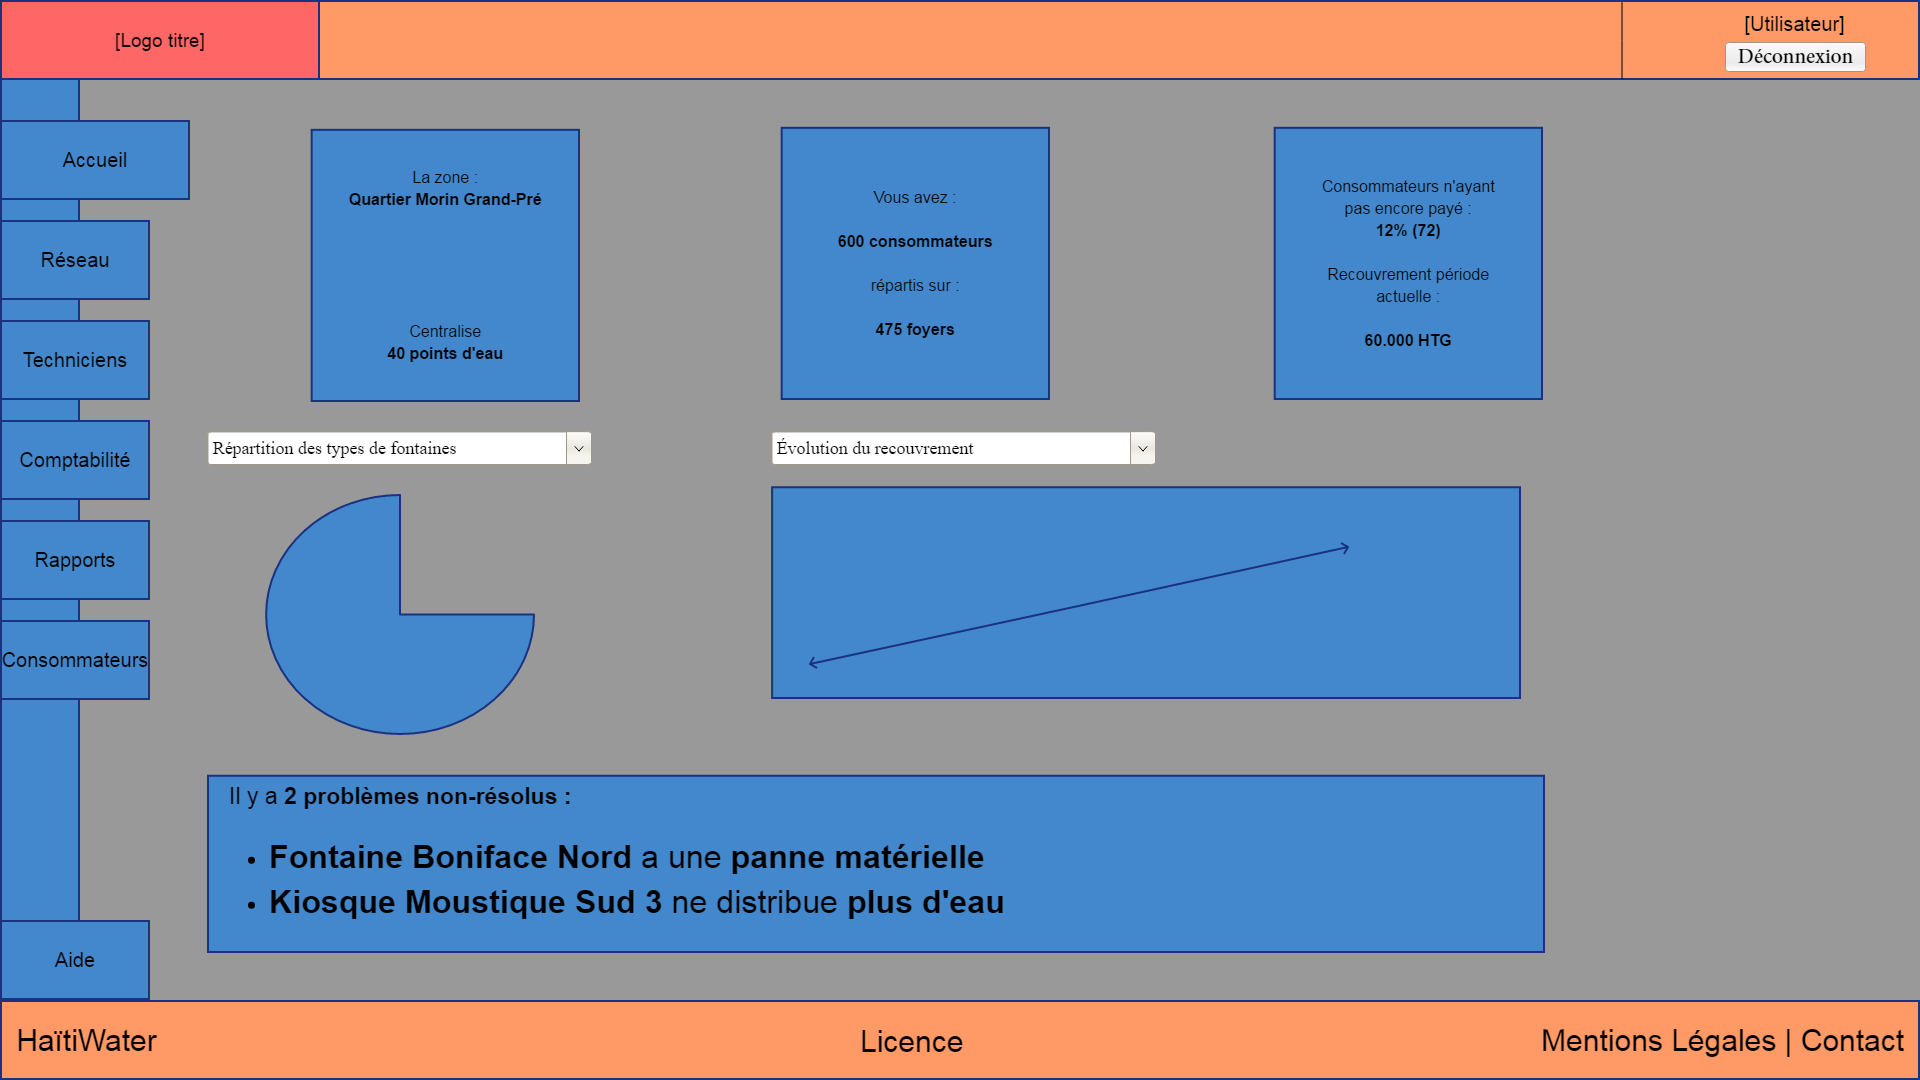
\includegraphics[width=.8\textwidth]{Cahier_des_Charges/accueil}
        \caption{\'Ecran d'accueil}
        \label{fig:zone_dashboard}
    \end{figure}

    Une fois identifié par son nom d'\gls{utilisateur} et mot de passe, l'\gls{utilisateur} arrive sur son tableau de bord. Le tableau de bord est personnalisé pour chaque type d'\gls{utilisateur} (gestionnaire de \gls{zone}, de \glspl{fontaine}, technicien/plombier).

    La figure~\ref{fig:zone_dashboard} présente le tableau de bord du gestionnaire de \gls{zone}. En en-tête, l'\gls{utilisateur} peut cliquer sur le logo de l'\gls{application} pour retourner à ce même tableau de bord à tout moment de sa navigation. Il peut aussi se déconnecter.

    À gauche, le menu principal indique à l'\gls{utilisateur} les pages auxquelles il peut accéder en cliquant sur les boutons. Le bouton étendu indique à l'\gls{utilisateur} sur quelle page il se trouve (ici "Accueil").

    Au centre, le contenu de la page propose tout d'abord trois \glspl{zone} informatives générales :
    \begin{itemize}
      \item \gls{zone} courante, son nom et le nombre de \glspl{point_eau} (kiosques, \glspl{fontaine}, \glspl{reservoir}, \glspl{prise_individuelle})
      \item \glspl{consommateur}, nombre de foyers
      \item Recettes, pourcentage de recouvrement des paiements, recettes totales
    \end{itemize}
    L'\gls{utilisateur} peut cliquer sur chacune des \glspl{zone} pour aller sur la page comprenant le détail des informations (respectivement les pages \emph{\gls{reseau}, \glspl{consommateur}, Comptabilité}).

    Ensuite, des graphiques sont proposés à l'\gls{utilisateur} (ici, la répartition des types de \glspl{point_eau} et l'évolution du taux de recouvrement en fonction du temps). L'\gls{utilisateur} peut utiliser la flèche à droite du titre du graphique pour en choisir un autre (quantité d'eau distribuée en fonction du mois, évolution du nombre de \glspl{consommateur}, ...).

    Enfin, une \gls{zone} de notification alerte l'\gls{utilisateur} des problèmes non-résolus sur le \gls{reseau} de distribution d'eau. Il peut également cliquer dessus pour aller à la page des problèmes.

  \subsection{Rapports et problèmes}
    \begin{figure}[H]
        \centering
        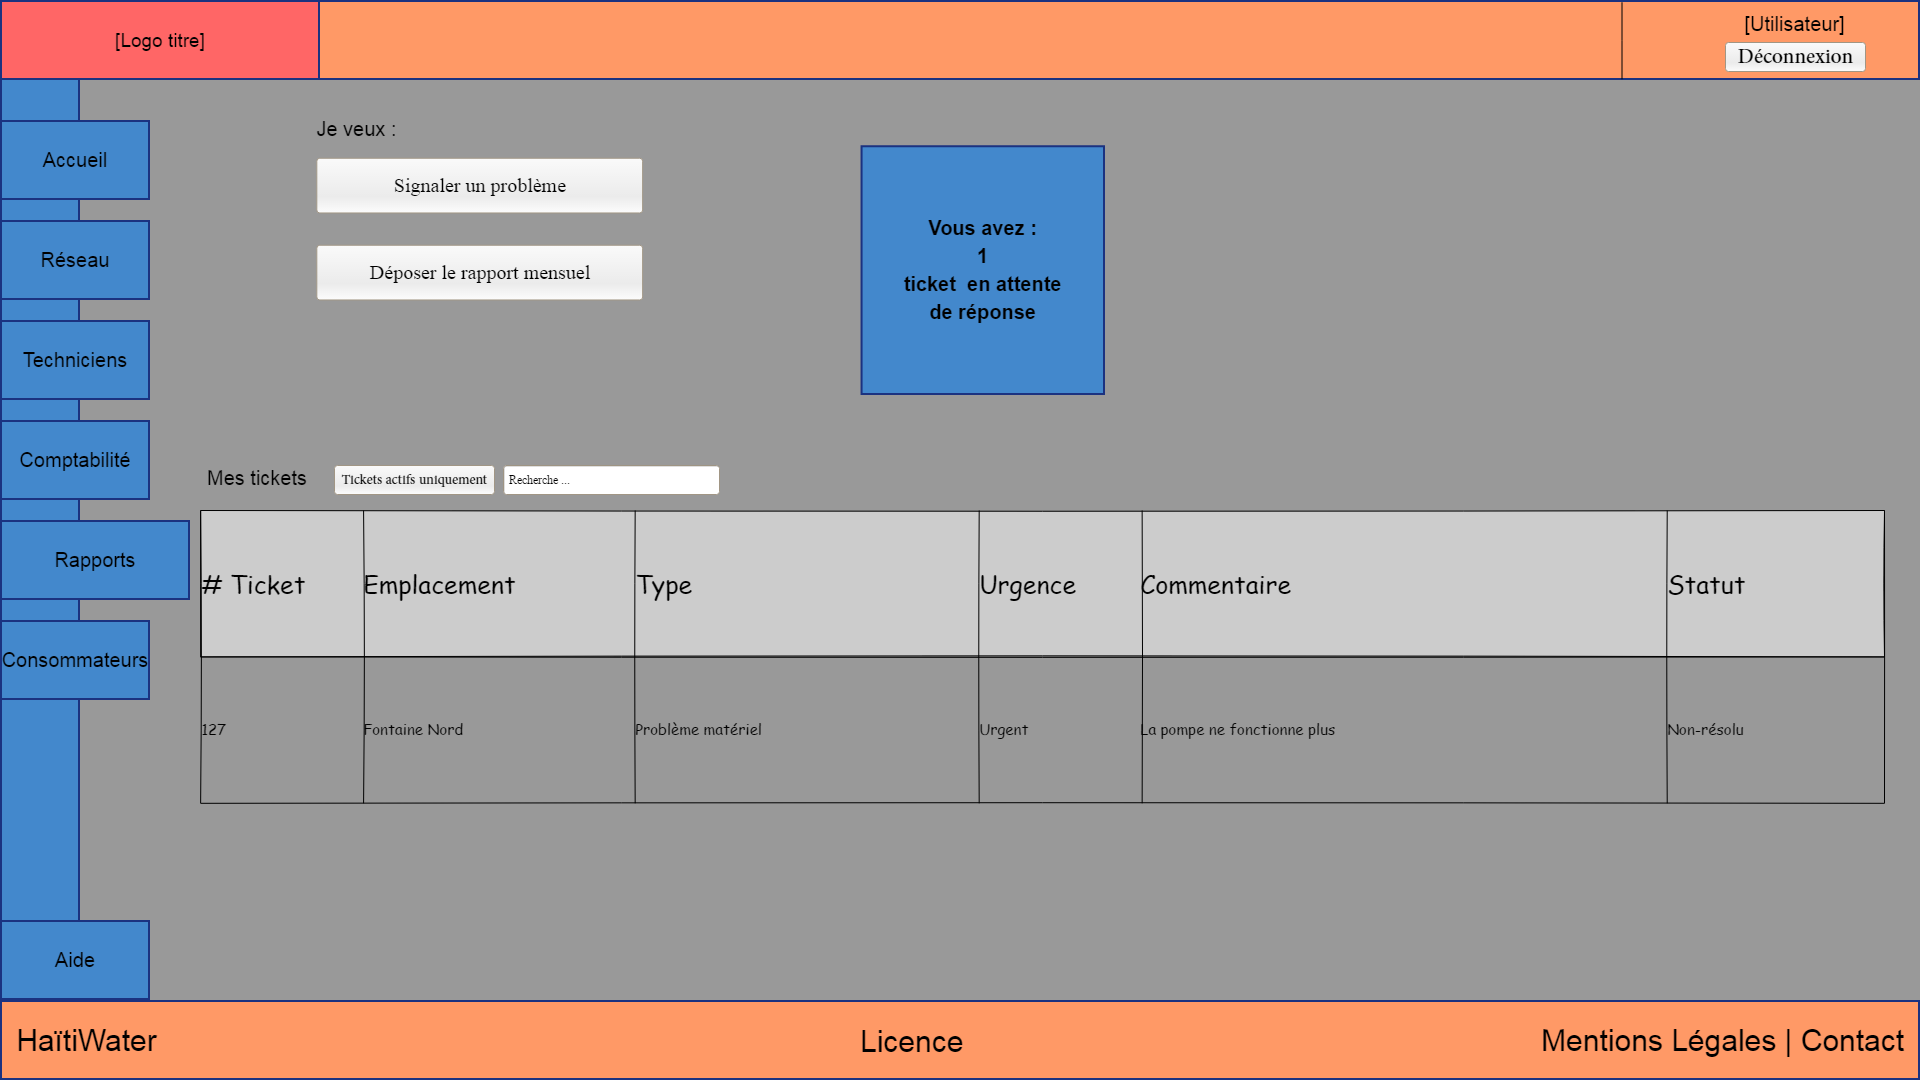
\includegraphics[width=.8\textwidth]{Cahier_des_Charges/rapports}
        \caption{\'Ecran des rapports}
        \label{fig:report}
    \end{figure}
    La figure~\ref{fig:report} présente la vue de rapport d'un gestionnaire de \gls{zone} et d'un gestionnaire de \glspl{fontaine}. Le gestionnaire peut signaler un problème ou déposer le \gls{rapport_mensuel} (voir figure~\ref{fig:monthly_report}).

    En dessous, le gestionnaire voit la liste de ses \glspl{ticket} en cours de traitement et leur statut. En cliquant dessus, il peut répondre aux messages du technicien/plombier (qui peut lui demander des précisions, proposer une solution, \dots). Des notifications alertent le gestionnaire lorsqu'il a reçu une réponse à son \gls{ticket}.

    \begin{figure}[H]
        \centering
        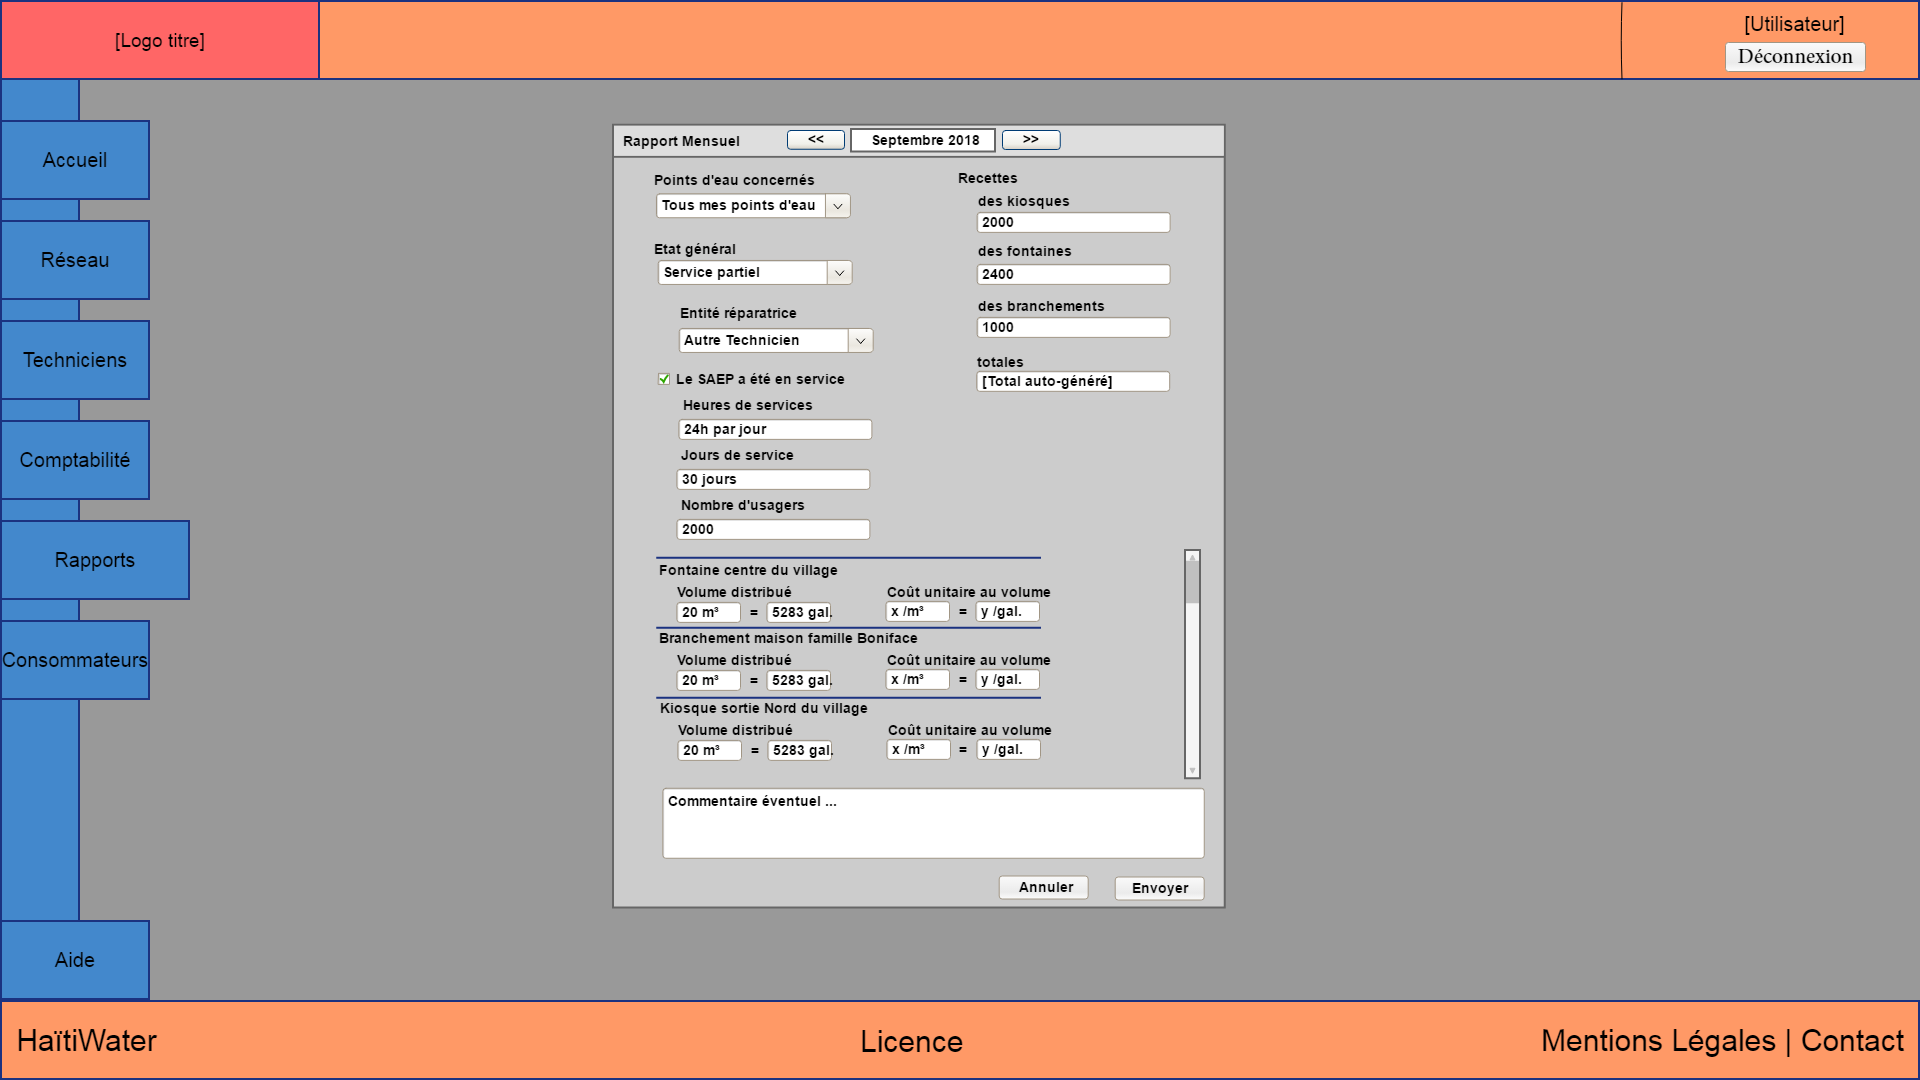
\includegraphics[width=.8\textwidth]{Cahier_des_Charges/rapports_mensuel}
        \caption{\gls{rapport_mensuel}}
        \label{fig:monthly_report}
    \end{figure}

    En figure~\ref{fig:monthly_report}, le gestionnaire fait son \gls{rapport_mensuel}. Chaque mois, ce formulaire doit être rempli pour obtenir les \glspl{donnee} du \gls{reseau}. Si un rapport a déjà été rempli (par exemple si le gestionnaire de \gls{zone} accède au \gls{rapport_mensuel} et qu'une partie des \glspl{donnee} a déjà été remplie par un gestionnaire de \glspl{fontaine}), il peut être modifié par ce même moyen.

    Ici, nous voyons le formulaire d'un gestionnaire de \glspl{fontaine}. Il se présente en cinq parties :
    \begin{itemize}
      \item Le gestionnaire de \glspl{fontaine} sélectionne la ou les sorties d'eau (\gls{fontaine}, \glspl{prise_individuelle}, kiosques, \glspl{reservoir}) parmis celles qui lui sont attribuées, pour lesquelles il souhaite faire son rapport.
      \item Le gestionnaire de \glspl{fontaine} indique s'il a pu être en service durant ce mois, si oui il indique le nombre de jours et d'heures durant lesquels le service était disponible.
      \item Le gestionnaire de \glspl{fontaine} indique les recettes pour les \glspl{fontaine}, kiosques et \glspl{prise_individuelle}, le total est affiché automatiquement.
      \item Pour chaque sortie d'eau sélectionnée au début du rapport, le gestionnaire de \glspl{fontaine} indique la quantité d'eau distribuée ainsi que les prix de distribution.
      \item Le gestionnaire de \glspl{fontaine} peut enfin ajouter un commentaire au \gls{rapport_mensuel}.
    \end{itemize}

    Le gestionnaire peut soumettre le rapport quand il le souhaite, même partiellement complété. Il peut y revenir plus tard et modifier les informations.

  \subsection{Vue du \gls{reseau}}
    \begin{figure}[H]
        \centering
        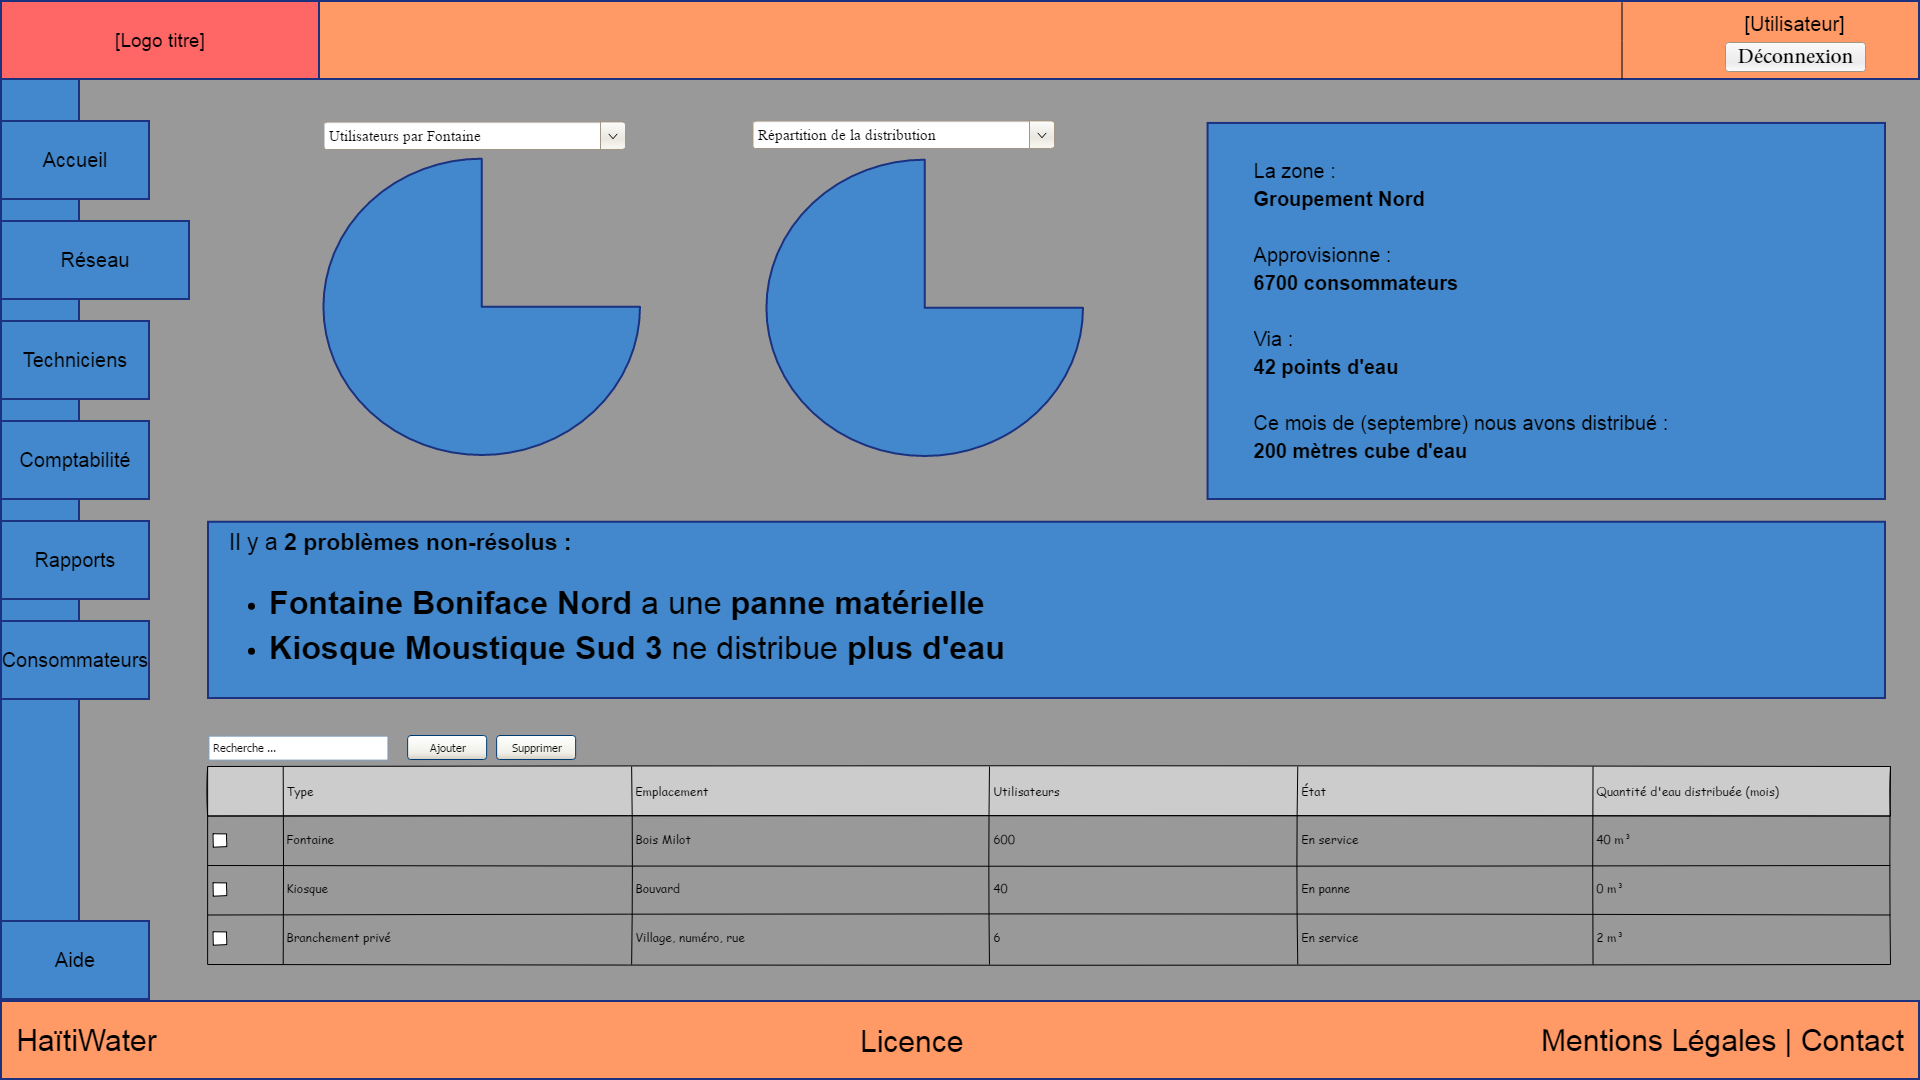
\includegraphics[width=.8\textwidth]{Cahier_des_Charges/reseau}
        \caption{Visuel du \gls{reseau}}
        \label{fig:network}
    \end{figure}
    La figure~\ref{fig:network} présente la vue d'accueil du \gls{reseau} de distribution. A partir de cette page, le gestionnaire de distribution ou de \glspl{fontaine} peut voir les installations du \gls{reseau} qui lui sont attribuées. Il y a à nouveau un espace dédié aux graphiques qu'il peut choisir et visualiser via la flèche à droite du titre.

    A droite, des informations générales sont disponibles ainsi que des statistiques (ici, en exemple, le volume mensuel total distribué).
    L'\gls{utilisateur} voit à nouveau un écran de notifications indiquant les problèmes qu'il faut résoudre.

\section{Besoins non-fonctionnels}
Dans cette section, nous allons détailler certaines caractéristiques souhaitables pour l'\gls{application}. Il s'agit d'exigences sur le \gls{systeme} en lui-même et pas sur ce qu'il fait.
\begin{enumerate}
  \item Sécurité des \glspl{donnee}.
  \item Fonctionnement sur périphérique mobile (tablettes et smartphones).
  \item Adaptabilité de l'interface graphique aux différentes tailles d'écrans.
  \item Présence d'une documentation qualitative pour les développeurs et les \glspl{utilisateur} du \gls{systeme}.
  \item \gls{application} \gls{scalable}, c'est-à-dire capable de fonctionner aussi bien avec les données des zones d'essai au début du \gls{deploiement}, que sur un nombre bien plus important de zones géographiques une fois les essais terminés.
  \item \gls{application} \gls{modulaire} pour permettre l'ajout de fonctionnalités futures.
\end{enumerate}
% Explication des besoins non-fonctionnels
\section{Approche \label{sec:approach}}
  Pour créer ce cahier des charges qui établit les fonctionnalités et le fonctionnement général de l'\gls{application}, nous avons utilisé les documents fournis par Protos et disponibles en ligne.
  \begin{description}
    \item[Les fichiers Excel,] au nombre de trois ont été principalement utilisés pour le choix des \glspl{donnee} et fonctionnalités de l'\gls{application}. Deux des fichiers concernent les \gls{caepa} et recensent leurs \glspl{fontaine}, \glspl{consommateur} et comptabilités à l'échelle annuelle. Un fichier expose au niveau national et mensuel l'état du \gls{reseau} (fonctionnement, quantités d'eau distribuées) et les recettes envoyées via formulaire par des \gls{tepac} qui gèrent le \gls{reseau} à leur échelle sur le terrain.
    \item[Les documents de contexte] envoyés par Protos faisant état de la situation en Haïti, le projet de Protos sur place et leur fonctionnement.
    \item[Le rapport de capitalisation] fourni récemment et expliquant le processus, pour Poste Métier, de fonctionnement de la distribution de l'eau.
  \end{description}
  Les fichiers Excel ont été notre plus grande source d'information puisqu'ils nous permettent de connaître le \gls{systeme} informatique actuel, quelles sont les \glspl{donnee}, comment sont-elles collectées et utilisées.
  Les fichiers de contexte ont permis de comprendre la situation, d'identifier les intervenants et risques de l'\gls{application}.
  Le rapport de Poste Métier a été très intéressant pour comprendre le fonctionnement précis d'une \gls{zone} du \gls{reseau} de distribution.

  Notre approche générale dans cette \gls{application} est d'automatiser la collecte et faciliter la gestion de toutes les \glspl{donnee} présentes dans les documents Excel actuellement utilisés en Haïti. Dans ce cahier des charges, nous présentons une \gls{application} hiérarchique où chaque \gls{utilisateur} fait remonter l'information dont il dispose (exactement comme le fonctionnement actuel des \glspl{donnee} Excel qui sont extraites des formulaires).

  \begin{shaded}
    Si ce cahier des charges vous semble incorrect (incompréhension d'une fonctionnalité) ou incomplet (manque de fonctionnalités), tout nouveau document permettant de mieux comprendre votre fonctionnement et vos désirs pour l'\gls{application} est le bienvenu.
  \end{shaded}

\section{Choix technolgiques}
  Conformément aux demandes, l'\gls{application} utilisera des technologies gratuites et aussi peu différentes que possible afin de ne pas requérir trop d'apprentissages différents. Les décisions des technologies utilisées dans le développement tentent de maximiser :
  \begin{description}
    \item[Popularité:] Plus une technologie est populaire, plus elle est susceptible d'être maintenue à jour, de disposer de guides et d'aides en ligne.
    \item[Simplicité:] Pour permettre aux futurs développeurs de l'\gls{application} de la maintenir à jour et de la faire évoluer avec un minimum de connaissances requises.
    \item[Performance:] Afin que l'\gls{application} soit utilisée le plus longtemps possible et qu'il ne soit pas nécessaire de recommencer à zéro à cause d'une technologie limitant l'\gls{application}.
  \end{description}

  Sur ces bases, nous avons déjà arrêté les choix généraux suivants :
  \begin{description}
    \item[\gls{interface}:] Les langages HTML5, CSS3 et JavaScript sont les plus populaires et peu d'alternatives existent pour le développement d'\gls{application}s internet, aucune n'étant aussi simple à utiliser.
    \item[\gls{application}:] Nous allons utiliser le framework\footnote{Framework : structure logicielle encadrant l'\gls{application}, permettant d'automatiser certaines phases du développement.} Django, le sixième plus populaire avec un score de 94\%\footnote{Statistique de https://hotframeworks.com/, septembre 2018.} et qui permet de programmer la logique de l'\gls{application} dans le langage Python, très populaire et adapté autant pour un débutant que pour un expert en programmation.
    \item[Base de \glspl{donnee}:] Pour stocker les \glspl{donnee}, nous allons utiliser la technologie SQL avec le \gls{systeme} de gestion PostgreSQL\footnote{Quatrième mondial selon https://db-engines.com/en/ranking.} qui présente l'énorme avantage d'avoir un module géographique (PostGIS) qui peut interagir directement avec le module géographique de l'\gls{application} (GeoDjango).
  \end{description}

\newpage

\appendix
\section{Vision détaillée des visuels d'écran \label{annexe}}
  \filbreak
  \begin{figure}[H] % normal figure to prevent section break
    \centering
    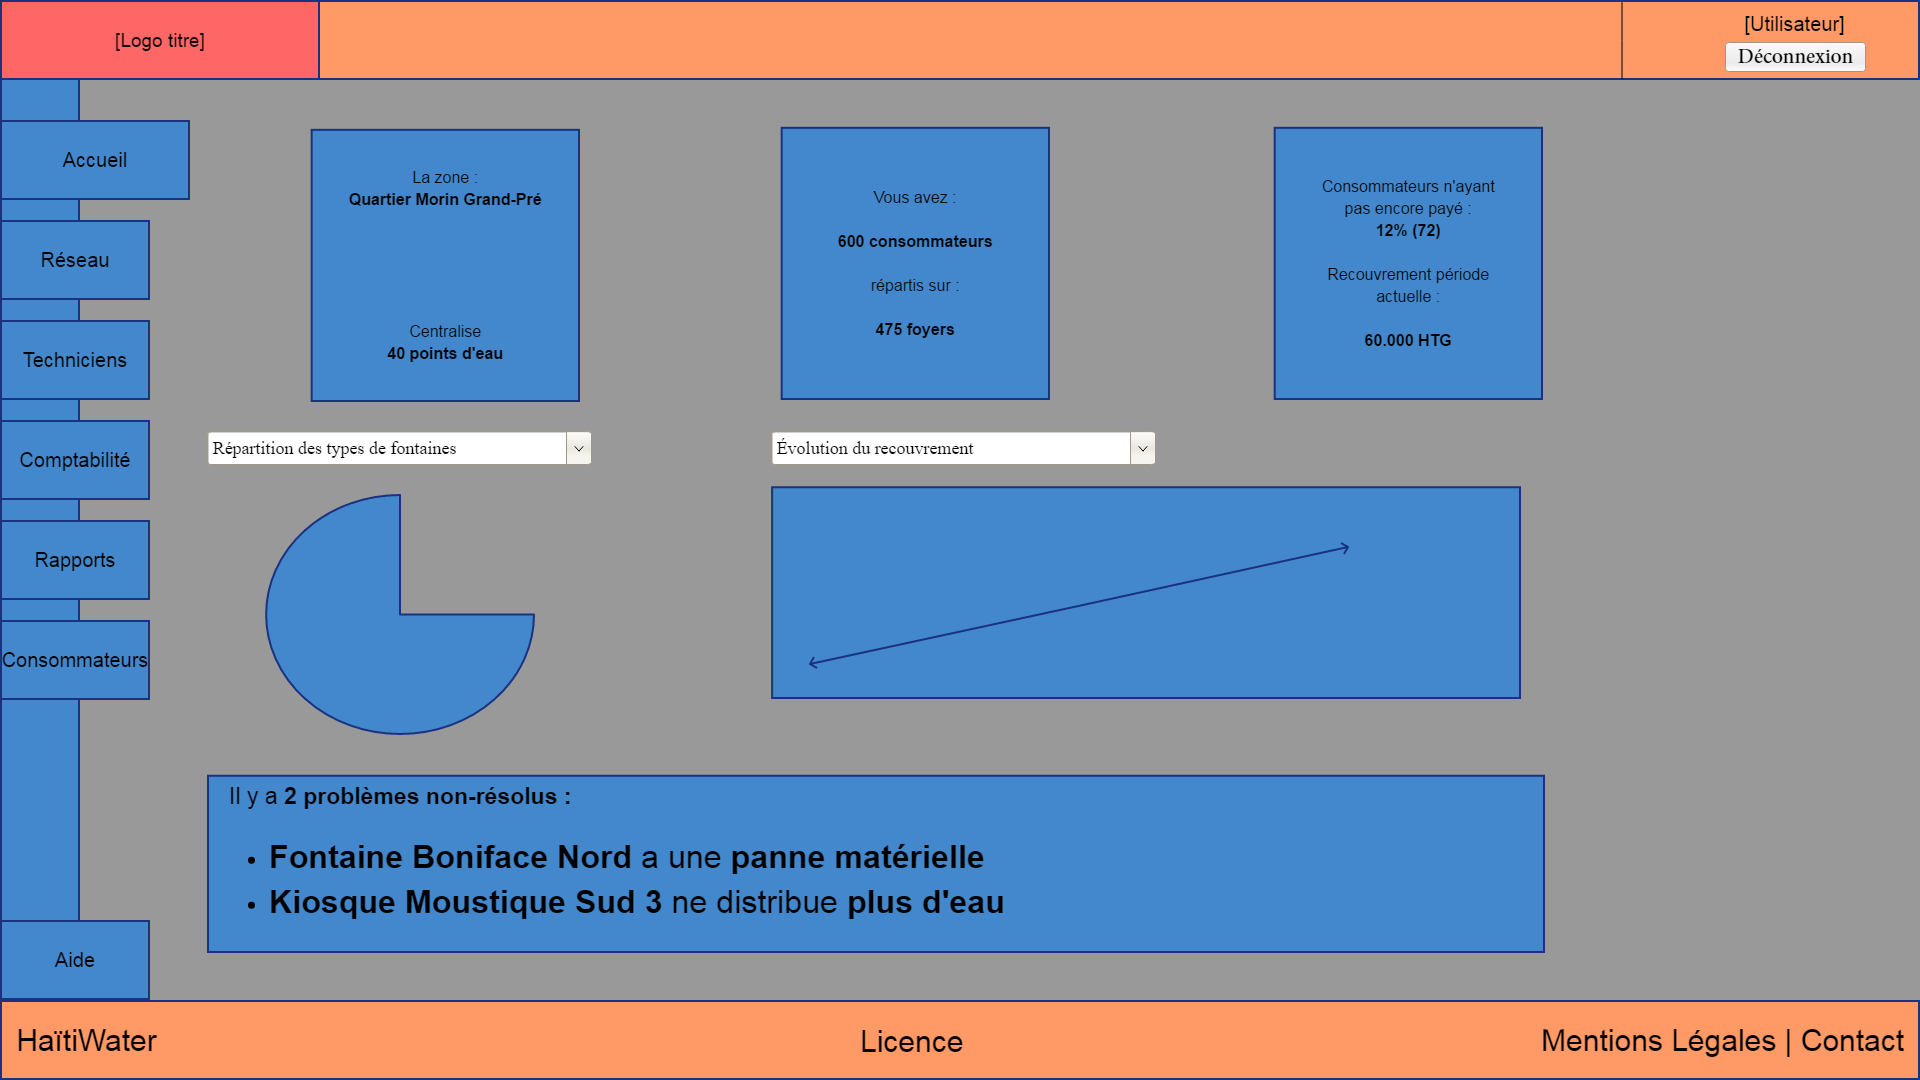
\includegraphics[scale=0.32, angle=90]{Cahier_des_Charges/accueil}
  \end{figure}

  \begin{sidewaysfigure}
    \centering
    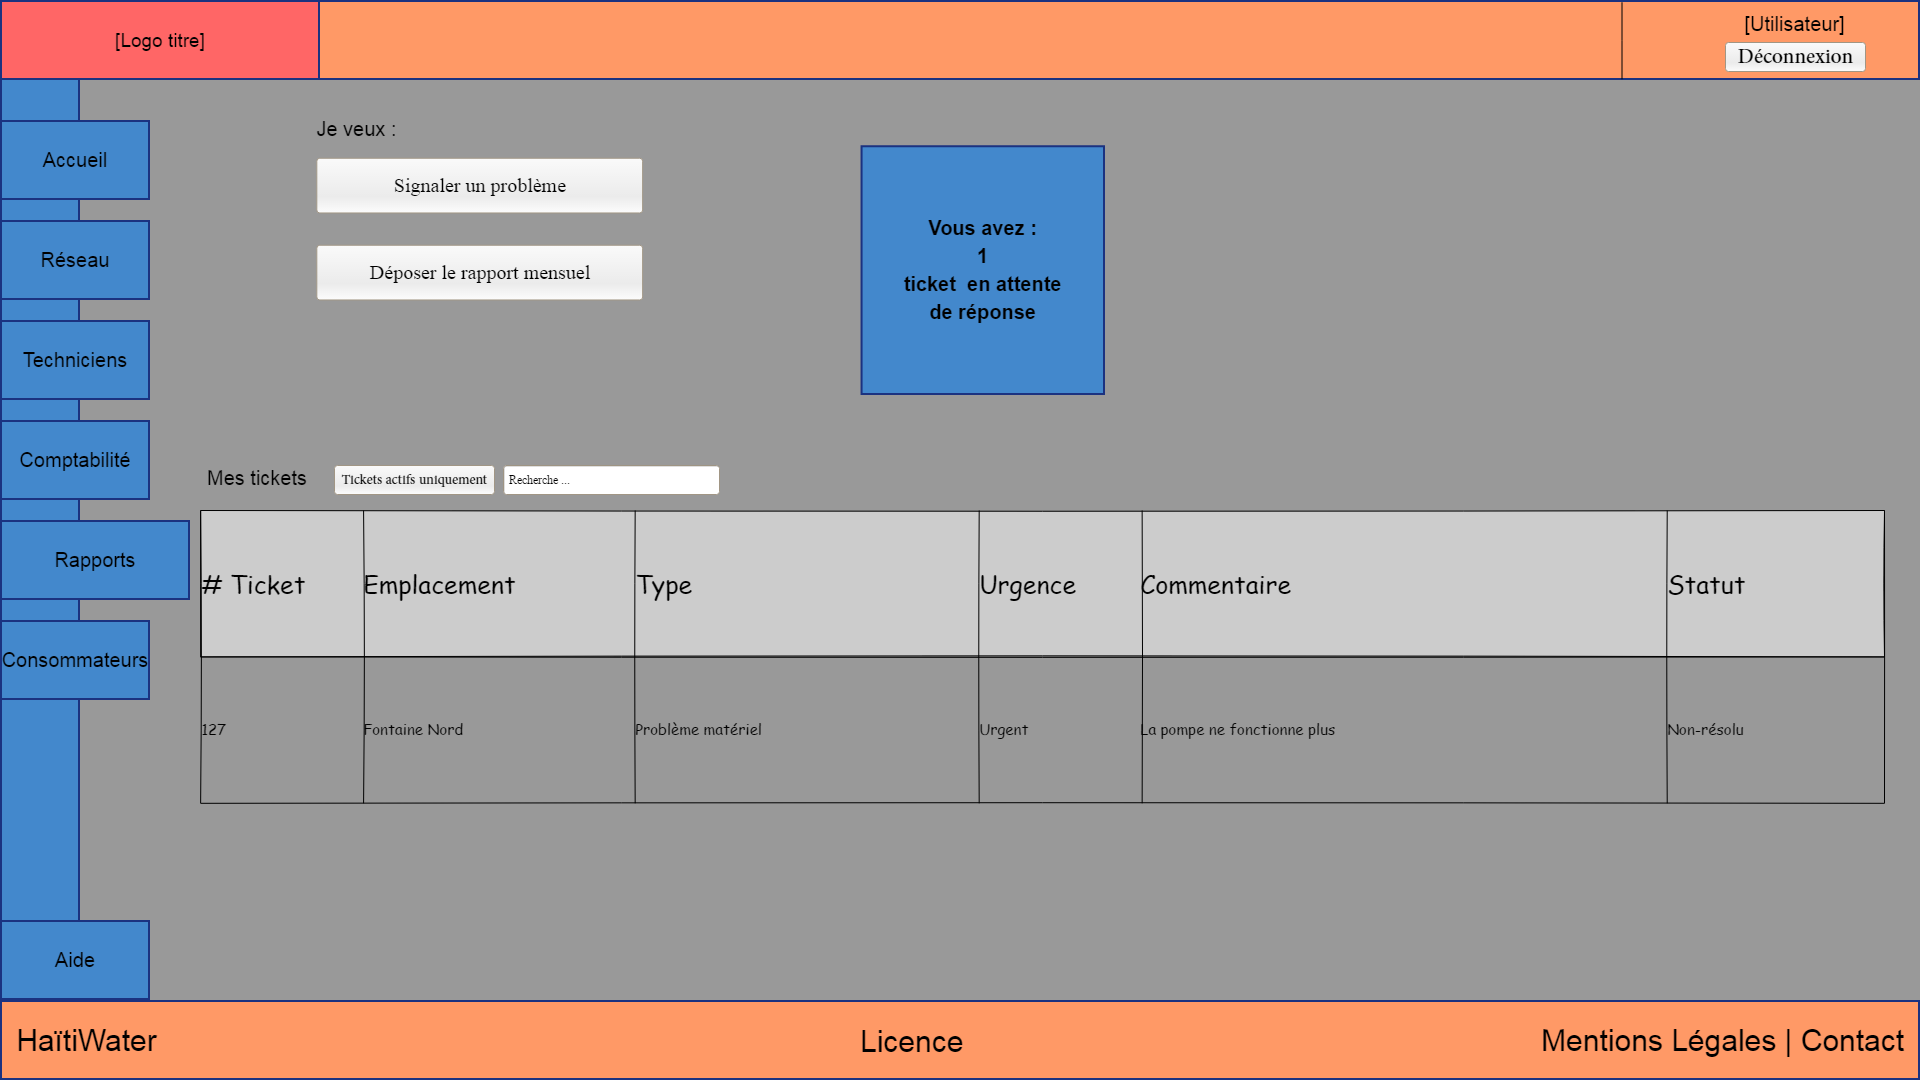
\includegraphics[width=\textwidth]{Cahier_des_Charges/rapports}
  \end{sidewaysfigure}

  \begin{sidewaysfigure}
    \centering
    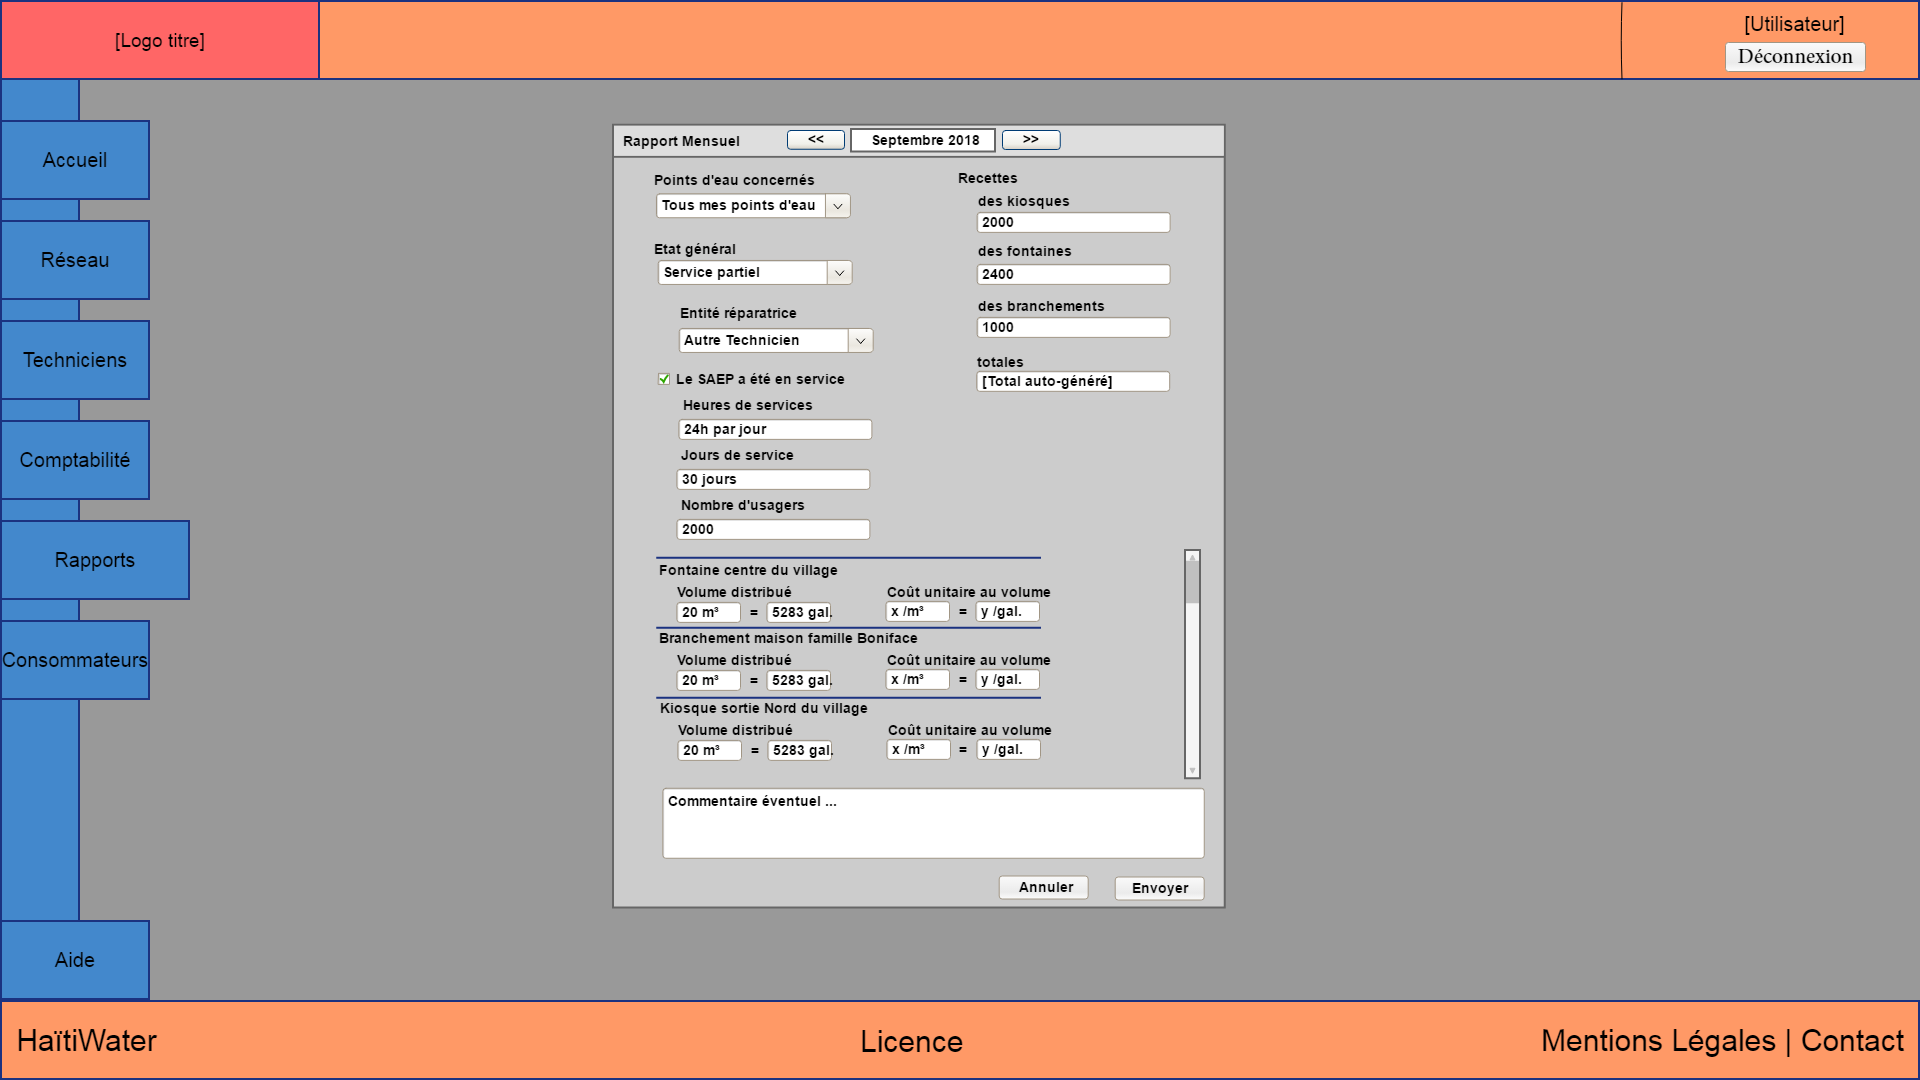
\includegraphics[width=\textwidth]{Cahier_des_Charges/rapports_mensuel}
  \end{sidewaysfigure}

  \begin{sidewaysfigure}
    \centering
    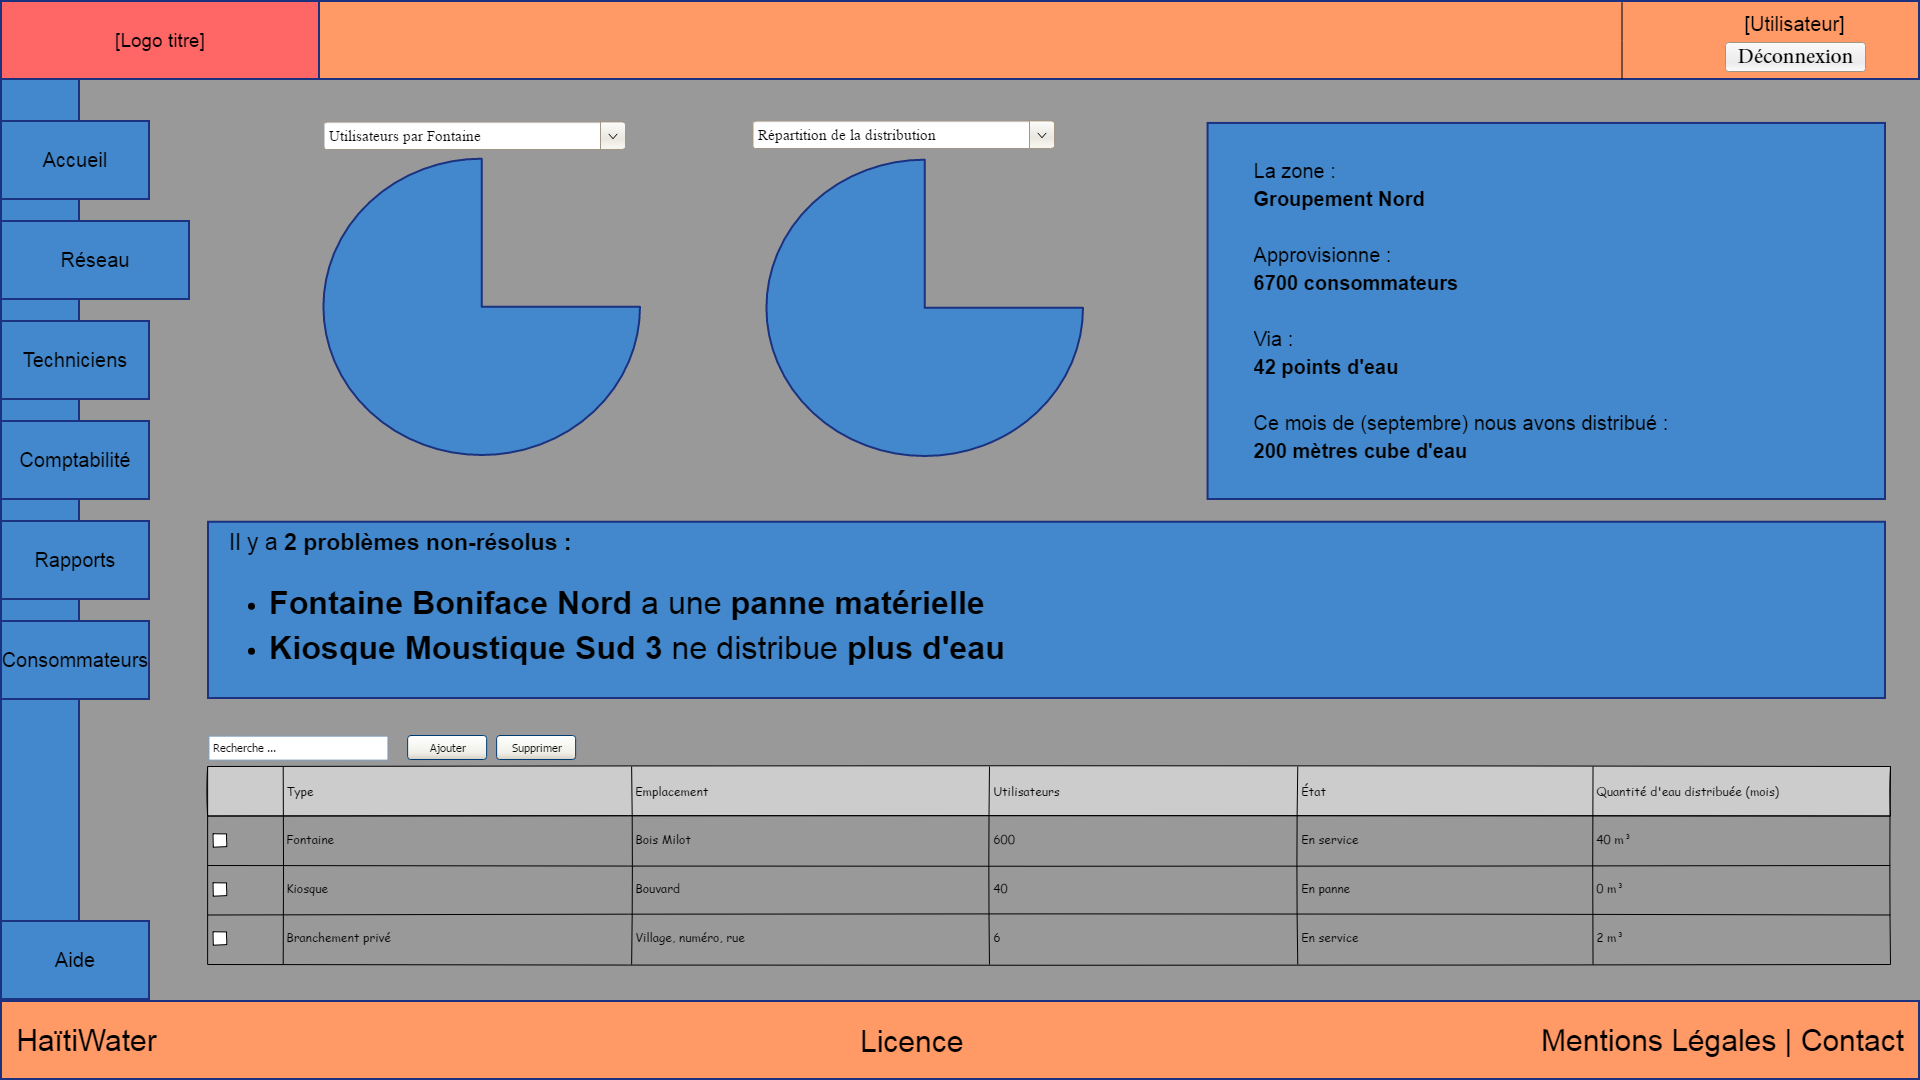
\includegraphics[width=\textwidth]{Cahier_des_Charges/reseau}
  \end{sidewaysfigure}

\end{document}
